{\color{gray}\hrule}
\begin{center}
\section{Intermediate/Preliminary Results}
%\textbf{Small description}
\end{center}

{\color{gray}\hrule}

% qua le figure degli istogrammi e del contrast stretching

\begin{multicols}{2}

\subsection{Pre-processing}
Our aim is to use pictures in non-optimal lighting and perspective conditions, so due to the fact that our training dateset (Dress-Code) is mainly composed of high quality professionaly taken images, we are trying to imitate this condition and apply some enhancement to the generic input picture. In particular we chose to use:

1. Constrast stretching: it is a simple image enhancement technique that attempts to improve the contrast in an image by stretching the range of intensity values it contains to span a desired range of values. Table \ref{contr_stretch} depicts a sample;

2. Bilateral filtering: we attempt to remove the noise while preserving the sharpeness of the edges. Table \ref{contr_stretch} depicts a sample;

3. Background removal: we discuss it in \ref{back_rem}.


\subsection{Background removal}\label{back_rem}
As our dataset training images usually possess a plain and homogeneous background, in order to decrease variance between training and real-world images, and to decrease the computational training effort, we are comparing semantic backgroud removal using different kind of segmentation techniques. Since this procedure is applied to real-world images, we trained a network over \textit{Full Body TikTok Dancing Dataset}\cite{tik_tok_dataset} that we belived to have a more natural picture acquisition of body shapes. To perform the semantic segmentation, we used U-Net network and, as of now, we have trained over 10 epochs as a trial. On the same dataset, we tested pre-trained Detectron2 and the "enhanced" Detectron2+GrabCut+MedianFilter module.	

The comparison between these solutions is depicted in the table \ref{comp_results}, as we can see the GrabCut module did not achieve better results than the raw Detectron2 module. The original intent of refining the shapes around the bodies was achieved, but a drawback of this method is that some parts of the shapes were lost as the algorithm did not recognize them as foreground. The numerical results are shown in the table \ref{comp_metrics}.

\end{multicols}

\FloatBarrier

% contrast stretching images
\begin{table}[hbt!]
\centering
\begin{tabular}{ccc}
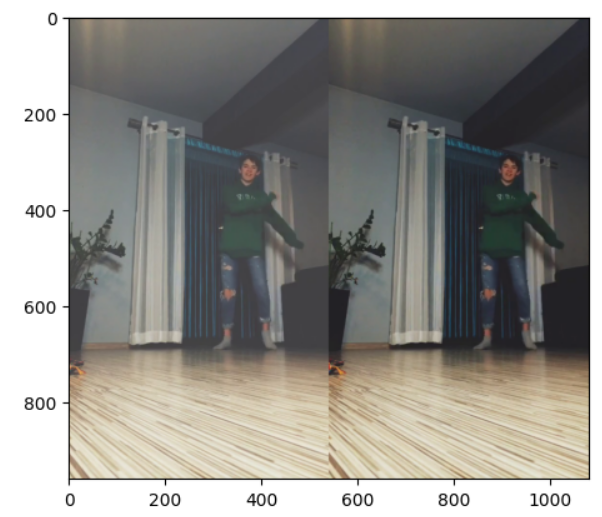
\includegraphics[width=.30\linewidth,valign=m]{constr_stretch} & 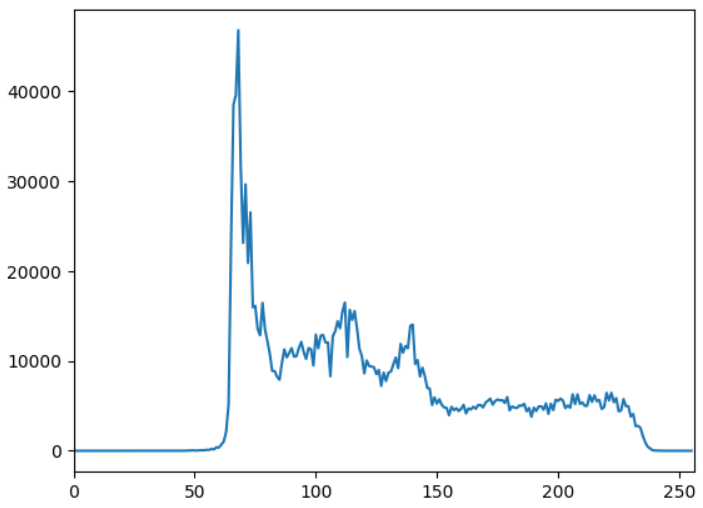
\includegraphics[width=.30\linewidth,valign=m]{hist_constr_stretch} & 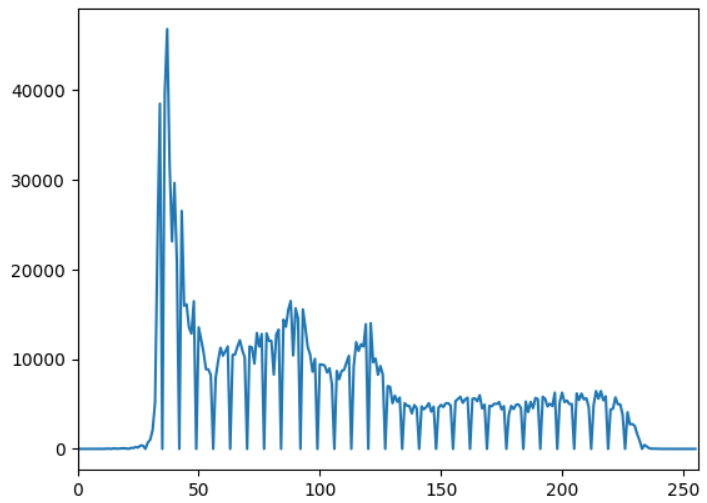
\includegraphics[width=.30\linewidth,valign=m]{hist_constr_stretch_1} 
\end{tabular}
\caption{\label{contr_stretch}Sample from Tik-Tok Segmentation Dataset pre-processed with contrast stretching.}
\end{table}

% bilateral filter image
\begin{table}[hbt!]
\centering
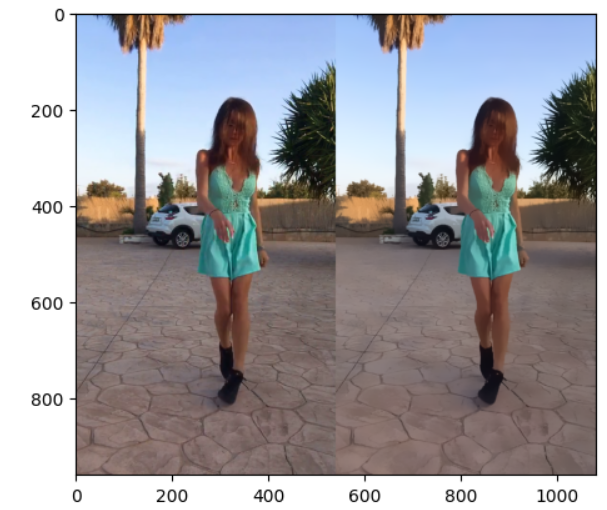
\includegraphics[width=.50\linewidth,valign=m]{bilateral_filtr}
\caption{\label{bil_fil}Sample from Tik-Tok Segmentation Dataset pre-processed with bilateral filter.}
\end{table}




\begin{table}[hbt!]
\centering
\begin{tabular}{ccccc}
Ground-truth & U-Net & Detectron2 & Detectron2 + GrabCut \\
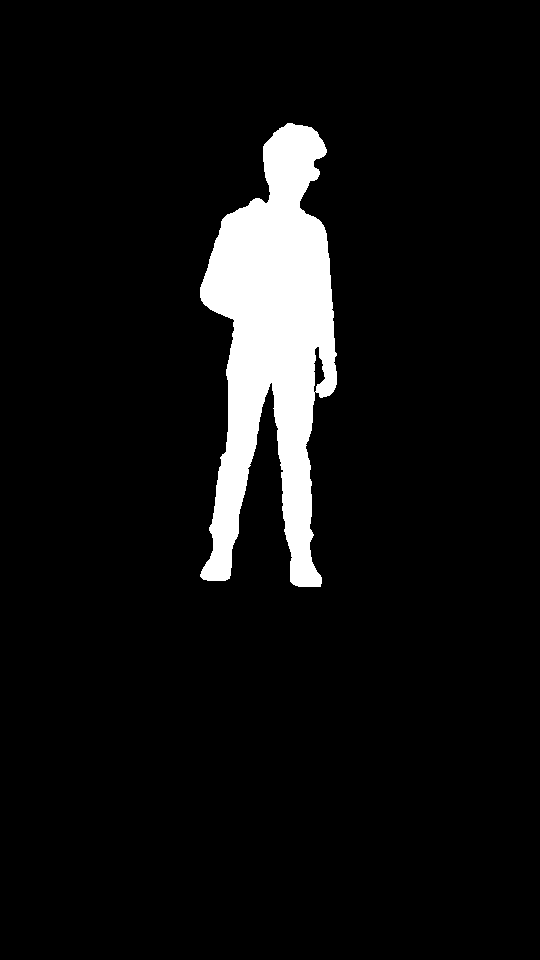
\includegraphics[width=.15\linewidth,valign=m]{ground-truth-result} & 
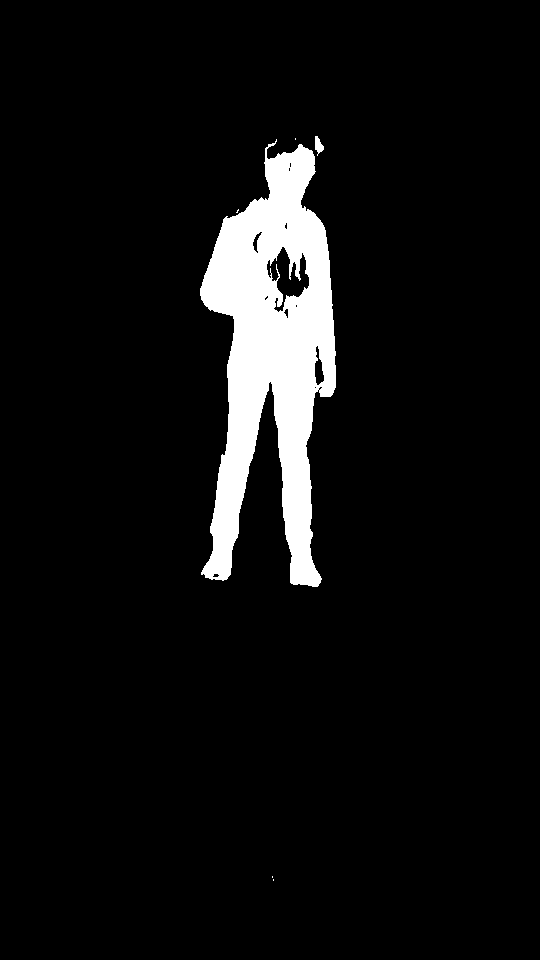
\includegraphics[width=.15\linewidth,valign=m]{unet-result} &
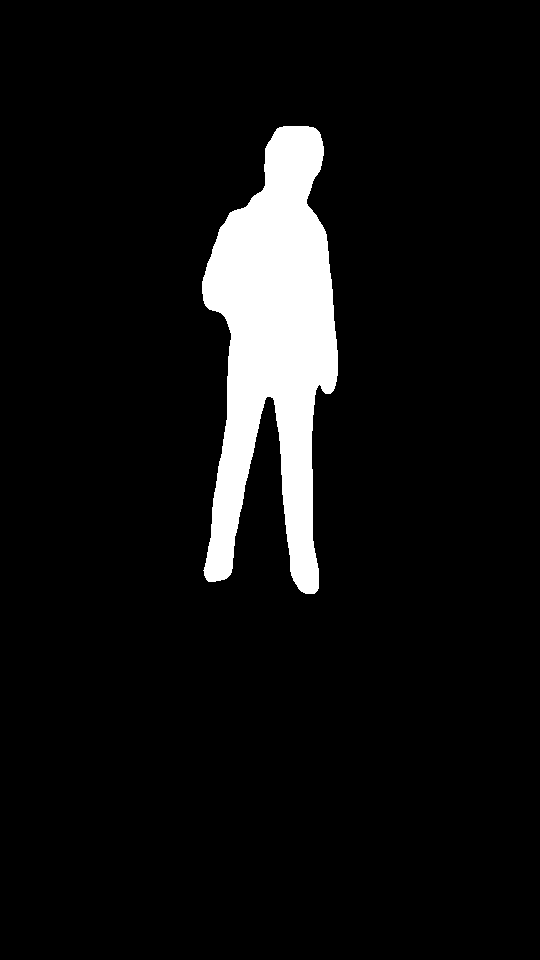
\includegraphics[width=.15\linewidth,valign=m]{detectron-result} &
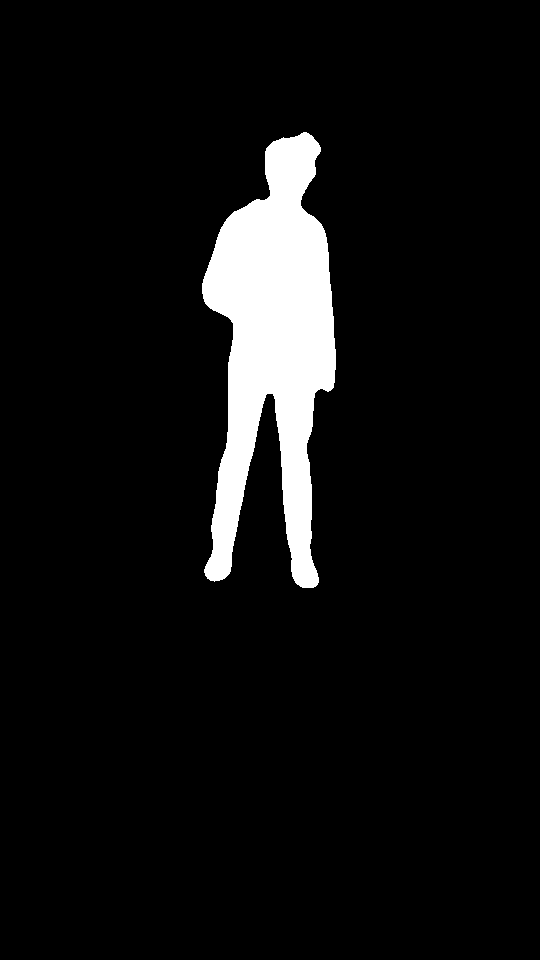
\includegraphics[width=.15\linewidth,valign=m]{detectron-grab-cut-result} \\
\end{tabular}

\caption{\label{comp_results}Samples of segmentation maps from Tik-Tok Segmentation Dataset.}
\end{table}


\begin{table}[hbt!]
\centering
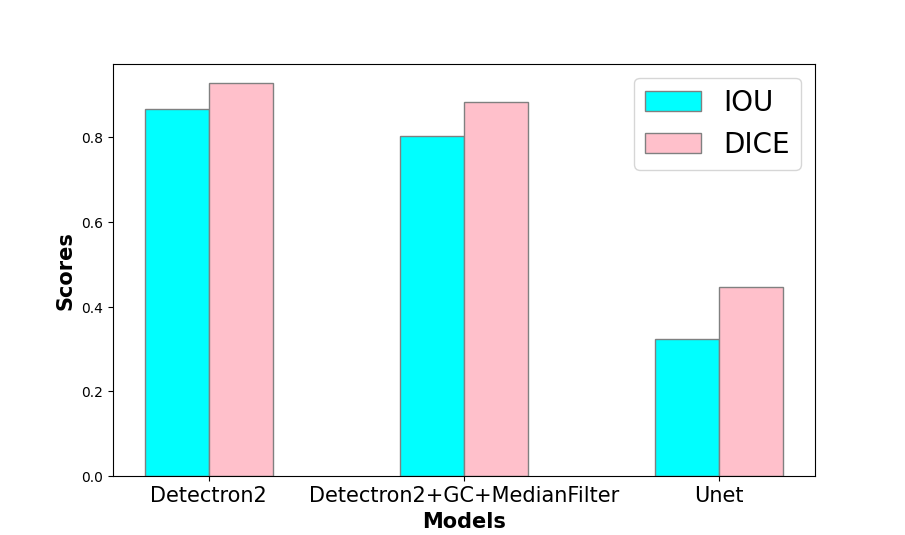
\includegraphics[width=1.1\linewidth,valign=m]{hist_results}

\caption{\label{comp_metrics}Comparison of IoU and DICE measures between our solutions of background removal.}
\end{table}



\FloatBarrier


\begin{multicols}{2}


\subsection{Garment retrieval}
As of now, we have tried to build a retrieval system based on the ORB algorithm with the following results:

\end{multicols}

\FloatBarrier
\begin{table}[hbt!]
\centering

\begin{tabular}{cc}
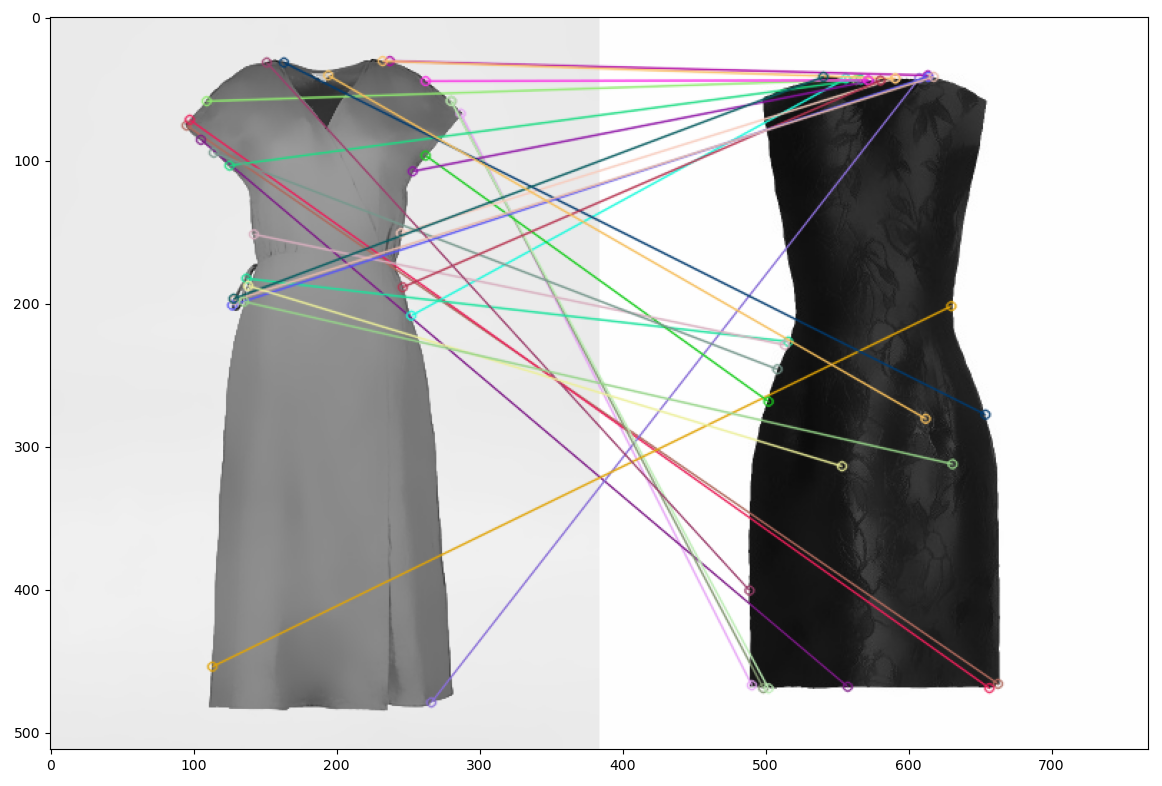
\includegraphics[width=.40\linewidth,valign=m]{orb_sample} & 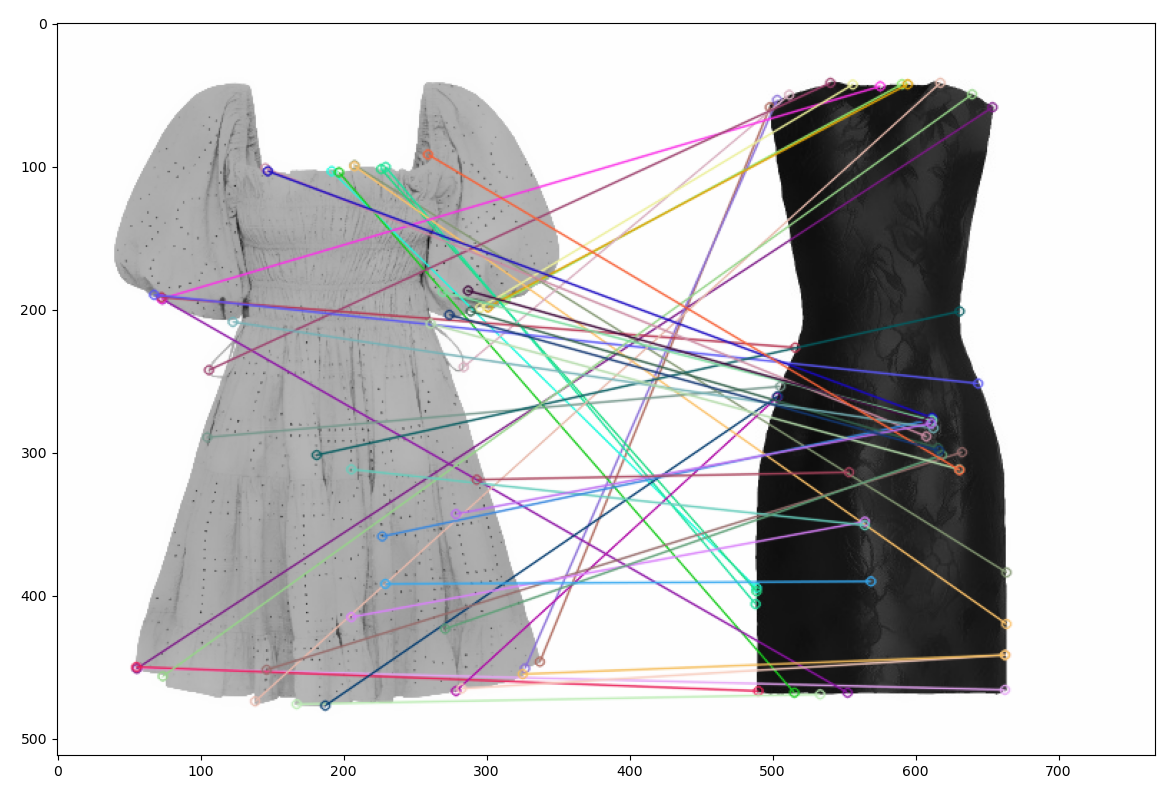
\includegraphics[width=.40\linewidth,valign=m]{orb_sample_1} \\
\end{tabular}

\caption{\label{orb_samples} Examples of keypoints matching between query images (left ones) and best match reference image (right ones).}

\end{table}
\FloatBarrier


\begin{multicols}{2}

\subsection{Conclusions}
Our try-on system is still very deep into the developmental phase, as such making assessments related to the time needed to complete the project and the potential emergence of future issues is difficult.
Although, given that our approach has been validated by state-of-the-art literature and that we have been advancing, little by little, towards achieving the project goals, our work may very well lead to a successful outcome.

\end{multicols}